\documentclass[11pt,a4paper]{article}
\usepackage[utf8]{inputenc}
\usepackage[T1]{fontenc}
\usepackage[spanish,es-noshorthands]{babel}
\usepackage{amsmath,amssymb,amsthm}
\usepackage{bm}
\usepackage{geometry}
\geometry{margin=2.5cm}
\usepackage{graphicx}
\graphicspath{{../figuras/}}
\usepackage{float}
\usepackage{xcolor}
\usepackage{hyperref}
\hypersetup{colorlinks=true,linkcolor=blue!50!black,citecolor=blue!50!black,urlcolor=blue!50!black}
\usepackage{enumitem}
\usepackage{booktabs}
\newtheorem{definition}{Definición}
\newtheorem{remark}{Observación}
\newcommand{\R}{\mathbb{R}}
\newcommand{\thetavec}{\bm{\theta}}
\newcommand{\transp}{^{\top}}
\newcommand{\promptIA}[1]{\begin{center}\fcolorbox{gray}{gray!8}{\parbox{0.9\linewidth}{\small\textbf{[FIGURA -- PROMPT IA]}\\[2pt]#1}}\end{center}}
\title{\textbf{M3 --- Integración numérica y costo computacional}\\[2pt]\large Cómo se resuelve una EDO en la computadora, y qué cuesta hacerlo}
\author{Proyecto Wilson--Cowan --- Iniciación a la I+D ITBA}
\date{\today}
\begin{document}
\maketitle
\tableofcontents
\bigskip

% ==========================================================================
\section*{Antes de empezar}
Este documento requiere \textbf{M2 (EDOs y sistemas dinámicos)}: damos por conocido qué es una EDO $\dot{\mathbf{x}}=f(\mathbf{x},t)$, qué es un flujo, el Jacobiano $\partial f/\partial\mathbf{x}$ y sus autovalores. Acá pasamos de ``la EDO tiene una solución'' a ``cómo obtengo esa solución en la computadora, y cuánto me cuesta''. Es la maquinaria numérica sobre la que se apoya toda la identificación del proyecto: cada vez que entrenamos la Neural ODE para recuperar los 10 parámetros de Wilson--Cowan (WC), por dentro hay un integrador corriendo miles de veces. Entender su costo es entender de dónde sale el tiempo de cómputo.

% ==========================================================================
\section{Cómo se resuelve una EDO en la computadora}
\label{sec:pasos}
Una EDO $\dot{\mathbf{x}}=f(\mathbf{x},t)$ dice cuál es la \emph{pendiente} del estado en cada punto, pero no da la trayectoria $\mathbf{x}(t)$ en forma cerrada salvo casos triviales. WC, con sus dos poblaciones acopladas y sigmoideas, no tiene solución analítica. La computadora la construye \textbf{a mano, en pasos discretos}.

\paragraph{La idea.} Partimos de una condición inicial $\mathbf{x}(t_0)=\mathbf{x}_0$ conocida y de una grilla temporal $t_0<t_1<t_2<\dots$ con paso $\Delta t=t_{n+1}-t_n$. En cada paso usamos la información de la pendiente $f$ para estimar hacia dónde se mueve el estado y avanzar un cachito:
\begin{equation}
  \mathbf{x}_{n+1}=\mathbf{x}_n + (\text{incremento basado en } f).
\end{equation}
El resultado es una \emph{secuencia} de puntos $\{\mathbf{x}_0,\mathbf{x}_1,\mathbf{x}_2,\dots\}$ que aproxima la trayectoria continua. La calidad de la aproximación depende de dos cosas: cuán chico es $\Delta t$ y cuán inteligente es la forma de estimar el incremento. Esos dos ejes definen a los \emph{métodos de integración}.

\begin{remark}
En el proyecto, ``resolver WC'' aparece por todos lados: para \emph{generar} los datos sintéticos, para \emph{simular} el modelo candidato dentro del entrenamiento (el \emph{rollout} de la Neural ODE) y para \emph{correr la planta} en el lazo de control (ver P4, neural\_ode). Todas esas veces se está avanzando en pasos $\Delta t$.
\end{remark}

% ==========================================================================
\section{Métodos: Euler, RK4 y paso adaptativo}
\label{sec:metodos}
La familia estándar es la de \textbf{Runge--Kutta}: métodos que estiman el incremento evaluando $f$ en uno o varios puntos dentro del paso y promediando esas pendientes \cite{hairer1993}.

\paragraph{Euler (orden 1).} El más simple: usa la pendiente al principio del paso y avanza recto.
\begin{equation}
  \mathbf{x}_{n+1}=\mathbf{x}_n+\Delta t\,f(\mathbf{x}_n,t_n).
\end{equation}
Una sola evaluación de $f$ por paso. Es barato pero \emph{tosco}: como extrapola con una recta, en una curva se va quedando ``por fuera'' y el error se acumula. Para lograr precisión decente hay que usar $\Delta t$ muy chico, y ahí lo barato por paso se paga en muchísimos pasos.

\paragraph{Runge--Kutta 4 (RK4, orden 4).} El caballito de batalla, y el que usa el proyecto. En cada paso evalúa $f$ en \textbf{cuatro puntos} (el inicio, dos estimaciones en el medio, y el final tentativo) y los combina con un promedio ponderado:
\begin{align}
  k_1 &= f(\mathbf{x}_n,\,t_n), &
  k_2 &= f\!\left(\mathbf{x}_n+\tfrac{\Delta t}{2}k_1,\;t_n+\tfrac{\Delta t}{2}\right),\notag\\
  k_3 &= f\!\left(\mathbf{x}_n+\tfrac{\Delta t}{2}k_2,\;t_n+\tfrac{\Delta t}{2}\right), &
  k_4 &= f\!\left(\mathbf{x}_n+\Delta t\,k_3,\;t_n+\Delta t\right),\notag\\
  \mathbf{x}_{n+1} &= \mathbf{x}_n+\tfrac{\Delta t}{6}\big(k_1+2k_2+2k_3+k_4\big).&&
  \label{eq:rk4}
\end{align}
Cuesta $4\times$ lo de Euler por paso, pero es tanto más preciso que compensa de sobra: con el \emph{mismo} $\Delta t$ el error es órdenes de magnitud menor. La Figura~\ref{fig:eulerrk4} muestra esta comparación sobre WC.

\paragraph{Paso fijo vs.\ adaptativo.} RK4 tal como está usa \emph{paso fijo}: el mismo $\Delta t$ de punta a punta. Esto es simple y predecible, pero derrocha esfuerzo en tramos donde la dinámica es suave y puede quedarse corto donde es abrupta. Los métodos de \textbf{paso adaptativo}, como \emph{Dormand--Prince} (el \texttt{ode45} de Matlab, también llamado RK45), \emph{estiman el error local} en cada paso comparando dos fórmulas de distinto orden y ajustan $\Delta t$ automáticamente: pasos grandes donde la solución es suave, chicos donde hay que resolver detalle fino. Ganan precisión por unidad de cómputo en problemas exigentes, a cambio de perder la regularidad de la grilla, que --- como veremos --- el proyecto necesita.

\begin{figure}[H]
\centering
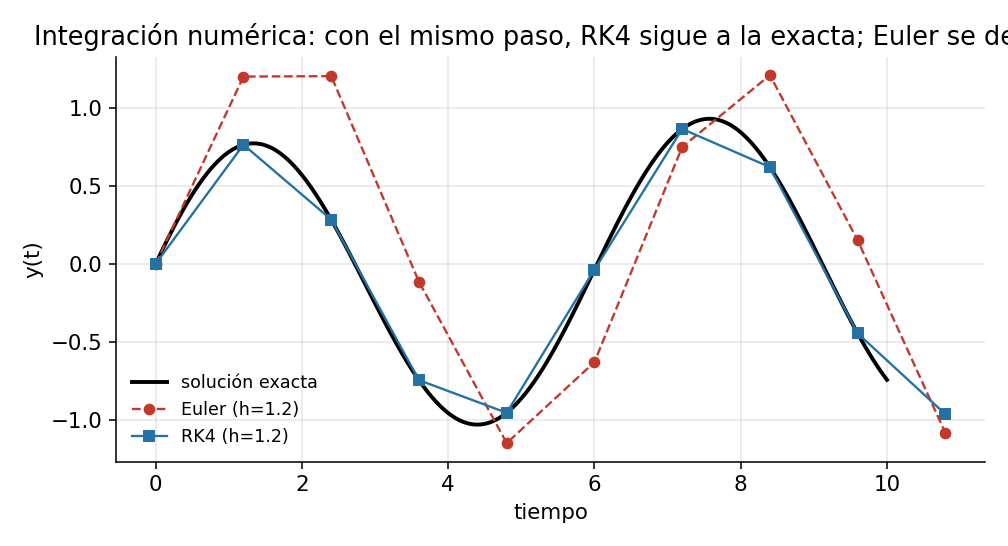
\includegraphics[width=0.75\linewidth]{fig_euler_rk4.png}
\caption{Integración de Wilson--Cowan con el mismo paso $\Delta t$: solución de referencia (exacta) frente a Euler y RK4. Euler se despega visiblemente de la curva verdadera; RK4 la sigue casi sin error. El costo por paso de RK4 es $4\times$ el de Euler, pero la ganancia de precisión es mucho mayor que $4\times$.}
\label{fig:eulerrk4}
\end{figure}

% ==========================================================================
\section{Error local, error global y orden}
\label{sec:error}
\begin{definition}[Error local y global]
El \textbf{error local} (o de truncamiento) es el que se comete en \emph{un} paso, suponiendo que se arrancó desde el valor exacto. El \textbf{error global} es el acumulado a lo largo de toda la trayectoria, tras muchos pasos.
\end{definition}

\begin{definition}[Orden de un método]
Un método es de \textbf{orden $p$} si su error global escala como $O(\Delta t^{p})$. Equivalentemente, su error local es $O(\Delta t^{p+1})$ (se pierde un orden al acumular sobre $\sim 1/\Delta t$ pasos).
\end{definition}

La consecuencia práctica es lo que importa: si \textbf{reduzco $\Delta t$ a la mitad},
\begin{itemize}[nosep]
  \item con \textbf{Euler} (orden 1) el error global cae $\sim 2\times$;
  \item con \textbf{RK4} (orden 4) el error global cae $\sim 2^{4}=16\times$.
\end{itemize}
Por eso el orden es tan valioso: un método de orden alto llega a la misma precisión con pasos mucho más grandes, es decir con \emph{menos pasos totales}. Esta es la palanca central de la próxima sección.

% ==========================================================================
\section{NFE: el costo como número de evaluaciones de \texorpdfstring{$f$}{f}}
\label{sec:nfe}
¿Cómo medir el costo de integrar sin depender del hardware, del lenguaje ni de cuán ocupada está la máquina? La medida estándar en la literatura de Neural ODEs \cite{chen2018} es el \textbf{NFE} (\emph{number of function evaluations}): cuántas veces se evalúa la función $f$ en total. Es una métrica limpia porque cada evaluación de $f$ es la operación cara (en el gray-box del proyecto, calcular las sigmoideas y el acoplamiento de WC), y el resto es aritmética barata.

Con \textbf{RK4 de paso fijo} el NFE es \emph{determinista}: como cada paso hace exactamente 4 evaluaciones,
\begin{equation}
  \boxed{\ \mathrm{NFE}=4\times(\text{n\'umero de pasos})\ }
\label{eq:nfe}
\end{equation}
y el número de pasos es $\approx T/\Delta t$ para un horizonte $T$. Escalando al entrenamiento completo:
\begin{equation}
  \mathrm{NFE}_{\text{total}}=4\times(\text{pasos por trayectoria})\times(\text{trayectorias})\times(\text{\'epocas}).
\end{equation}
De acá sale la conclusión operativa del proyecto: en identificación \emph{pura} sobre datos de WC corremos con la corrección neuronal apagada, así que el ``modelo'' son apenas $\sim\!10$ escalares y su costo es despreciable; \textbf{el costo real vive en la integración}, no en el tamaño de la red. Duplicar $\Delta t$ divide el NFE por dos, de forma directa y medible (ver M5 para el detalle de la arquitectura).

% ==========================================================================
\section{Rigidez, paso estable y la salvedad de los estímulos conmutados}
\label{sec:rigidez}
Si bajar $\Delta t$ mejora la precisión y subirlo abarata el cómputo, ¿qué impide poner $\Delta t$ enorme? Dos límites: la \emph{precisión} que exijamos y, sobre todo, la \textbf{rigidez} (\emph{stiffness}) del sistema.

\paragraph{Rigidez.} Un sistema es rígido cuando conviven escalas de tiempo muy dispares: modos que decaen rapidísimo junto a modos lentos. Se cuantifica con los autovalores del Jacobiano de estado $\partial f/\partial\mathbf{x}$: la \emph{razón de rigidez} $|\lambda_{\max}|/|\lambda_{\min}|$ mide ese contraste. Cuanto más rígido, más chico debe ser $\Delta t$ para que un método explícito como RK4 sea \emph{estable} (si no, la solución numérica oscila o diverge aunque la real sea mansa) \cite{kim2021}. Nótese el paralelo con M4 (Fisher+SVD): allá el espectro de una sensibilidad a \emph{parámetros} predice identificabilidad; acá el espectro del Jacobiano de \emph{estado} predice el costo de integración. Misma idea, distinta derivada.

\paragraph{WC es poco rígido.} Sus dos constantes de tiempo ($\tau_e=1$, $\tau_i=2$) son del mismo orden: no hay separación brutal de escalas. Por eso WC \textbf{admite pasos grandes}: bajar la resolución temporal reduce el costo casi sin perder calidad \emph{en estímulos suaves}. Medido en el proyecto: se pasó de $\Delta t=0{,}05$ a $\Delta t=0{,}2$ (4$\times$ menos pasos), con el tiempo por época cayendo de $\sim\!510$\,ms a $\sim\!140$\,ms, sin degradar la identificación. Se evaluó además un solver adaptativo: \emph{no aporta}, precisamente porque WC no es rígido y no hay tramos que justifiquen refinar el paso.

\paragraph{Salvedad: estímulos conmutados.} Acá está el hallazgo fino del proyecto, y por qué el paso grande no es gratis siempre. Los estímulos $P(t),Q(t)$ que buscamos --- pensados para ser realizables con optogenética --- suelen ser \textbf{conmutados}: pulsos, escalones, \emph{on/off}. Entre muestras, el estímulo se mantiene constante mediante un \emph{retenedor de orden cero} (ZOH). En cada \textbf{conmutación} (cada flanco del estímulo) hay una discontinuidad, y el ZOH la ubica sobre la grilla con un error que no mejora con el orden del método: es de orden bajo por construcción. Con $\Delta t$ grande esos flancos quedan mal alineados en el tiempo y el error se acumula justo donde la dinámica lleva la información que más excita al sistema. Resultado medido: con estímulos conmutados a $\Delta t\approx 0{,}2$, la identificación \textbf{colapsa} (el error de $w_{II}$ trepa a 250--400\,\%). La regla práctica queda entonces partida: \textbf{$\Delta t$ grande solo para estímulos suaves / de banda limitada} (p.\,ej.\ un \emph{chirp}); \textbf{$\Delta t$ fino cuando el estímulo conmuta}. La Figura~\ref{fig:costdt} muestra este trade-off medido.

\begin{figure}[H]
\centering
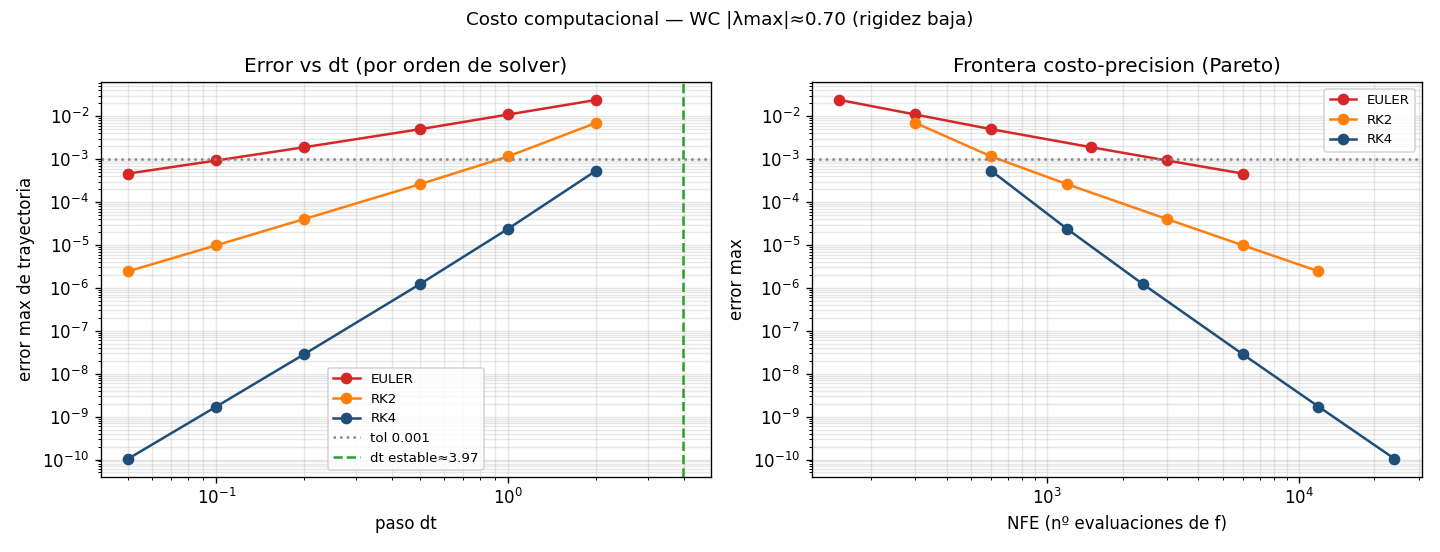
\includegraphics[width=0.75\linewidth]{cost_dt_sweep.png}
\caption{Costo computacional vs.\ paso de integración $\Delta t$ (figura del proyecto). Subir $\Delta t$ baja monótonamente el costo (menos pasos, menos NFE), pero la calidad se sostiene solo mientras el estímulo sea suave; con estímulos conmutados hay un $\Delta t$ máximo por debajo del cual hay que quedarse para no romper la identificación.}
\label{fig:costdt}
\end{figure}

% ==========================================================================
\section{Por qué el integrador tiene que ser diferenciable}
\label{sec:diferenciable}
Hasta acá integramos para \emph{simular}. Pero en el proyecto integrar es un medio para un fin mayor: \textbf{entrenar}. La Neural ODE aprende los parámetros $\thetavec$ minimizando el error entre la trayectoria simulada y la medida,
\begin{equation}
  \mathcal{L}(\thetavec)=\big\lVert\,\mathrm{rollout}(f_{\thetavec},\mathbf{x}_0,P,Q,\Delta t)-\mathbf{y}_{\text{medido}}\,\big\rVert^2,
\end{equation}
y para minimizar por descenso de gradiente necesitamos $\partial\mathcal{L}/\partial\thetavec$. El problema: $\mathcal{L}$ no depende de $\thetavec$ directamente, sino \emph{a través del integrador}. El gradiente tiene que \textbf{atravesar todo el solver}.

Acá es donde \eqref{eq:rk4} paga: RK4 es una \emph{composición de operaciones diferenciables} (sumas, productos, evaluaciones de $f$, que a su vez son sigmoideas suaves). Entonces la regla de la cadena --- la \emph{backpropagation} --- puede recorrer los cientos de pasos del \emph{rollout} hacia atrás y entregar el gradiente exacto respecto de $\thetavec$. Un integrador ``de caja negra'' (una rutina compilada que solo devuelve números) rompería esta cadena; por eso el proyecto usa un integrador \textbf{diferenciable}, escrito en un framework de autograd. Esto es lo que convierte a la integración numérica de una mera herramienta de simulación en el \emph{motor} del aprendizaje, y es el punto de contacto con M5, donde se desarrolla la arquitectura Neural ODE / PINN y el uso de \emph{multiple shooting} para que ese gradiente a lo largo de trayectorias largas no explote.

% ==========================================================================
\begin{thebibliography}{9}
\bibitem{hairer1993} E.~Hairer, S.~P.~Nørsett y G.~Wanner, \emph{Solving Ordinary Differential Equations I: Nonstiff Problems}, 2.\textsuperscript{a} ed., Springer, 1993.
\bibitem{chen2018} R.~T.~Q.~Chen, Y.~Rubanova, J.~Bettencourt y D.~Duvenaud, ``Neural Ordinary Differential Equations'', \emph{NeurIPS}, 2018.
\bibitem{kim2021} S.~Kim \emph{et al.}, ``Stiff neural ordinary differential equations'', \emph{Chaos}, 31(9):093122, 2021.
\end{thebibliography}

\end{document}
